\documentclass{beamer}
\usepackage[utf8]{inputenc}

\usetheme{Madrid}
\usecolortheme{default}
\usepackage{amsmath,amssymb,amsfonts,amsthm}
\usepackage{txfonts}
\usepackage{tkz-euclide}
\usepackage{listings}
\usepackage{adjustbox}
\usepackage{array}
\usepackage{tabularx}
\usepackage{gvv}
\usepackage{lmodern}
\usepackage{circuitikz}
\usepackage{tikz}
\usepackage{graphicx}

\setbeamertemplate{page number in head/foot}[totalframenumber]

\usepackage{tcolorbox}
\tcbuselibrary{minted,breakable,xparse,skins}



\definecolor{bg}{gray}{0.95}
\DeclareTCBListing{mintedbox}{O{}m!O{}}{%
  breakable=true,
  listing engine=minted,
  listing only,
  minted language=#2,
  minted style=default,
  minted options={%
    linenos,
    gobble=0,
    breaklines=true,
    breakafter=,,
    fontsize=\small,
    numbersep=8pt,
    #1},
  boxsep=0pt,
  left skip=0pt,
  right skip=0pt,
  left=25pt,
  right=0pt,
  top=3pt,
  bottom=3pt,
  arc=5pt,
  leftrule=0pt,
  rightrule=0pt,
  bottomrule=2pt,

  colback=bg,
  colframe=orange!70,
  enhanced,
  overlay={%
    \begin{tcbclipinterior}
    \fill[orange!20!white] (frame.south west) rectangle ([xshift=20pt]frame.north west);
    \end{tcbclipinterior}},
  #3,
}
\lstset{
    language=C,
    basicstyle=\ttfamily\small,
    keywordstyle=\color{blue},
    stringstyle=\color{orange},
    commentstyle=\color{green!60!black},
    numbers=left,
    numberstyle=\tiny\color{gray},
    breaklines=true,
    showstringspaces=false,
}
%------------------------------------------------------------
%This block of code defines the information to appear in the
%Title page
\title %optional
{1.9.17}
\date{August  2025}
%\subtitle{A short story}

\author % (optional)
{J.NAVYASRI- EE25BTECH11028}



\begin{document}
% Question Slide
\begin{frame}{Question}
\textbf{Question:} \\
Write the coordinates of a point \(\mathbf{P}\) on the \(x\)-axis which is equidistant from the points \(\mathbf{A(-2, 0)}\) and \(\mathbf{B(6, 0)}\).
\end{frame}

% Step 1: Theoretical solution
\begin{frame}{Theoretical solution}
Let the point $P$ be on the $x$-axis with coordinates:
\begin{equation}
P(x, 0)
\end{equation}

Since $P$ is equidistant from $A$ and $B$, their distances from $P$ are equal:
\begin{equation}
PA = PB
\end{equation}

\end{frame}

% Step 2: Theoretical solution 
\begin{frame}{Distance Formula}
Using the distance formula:
\begin{equation}
\sqrt{(x + 2)^2 + (0 - 0)^2} = \sqrt{(x - 6)^2 + (0 - 0)^2}
\end{equation}

This simplifies to:
\begin{equation}
|x + 2| = |x - 6|
\end{equation}

\end{frame}

% Step 3: Solve Cases
\begin{frame}{Solving Cases}
\textbf{Case 1:}
\begin{equation}
x + 2 = x - 6 \quad \Rightarrow \quad 2 = -6 \quad \text{(Not possible)}
\end{equation}

\textbf{Case 2:}
\begin{equation}
x + 2 = -(x - 6) 
\end{equation}
\[ x + 2 = -x + 6 \] 
\[ 2x = 4 \quad \Rightarrow \quad x = 2 \]
\end{frame}

% Final Answer
\begin{frame}{Answer}
Therefore, the coordinates of point $P$ are:
\begin{equation}
\boxed{(2, 0)}
\end{equation}
\end{frame}

\begin{frame}[fragile]
    \frametitle{Python Code}
    \begin{lstlisting}
import matplotlib.pyplot as plt

# Define points
A = (-2, 0)
B = (6, 0)
P = (2, 0)

# Create figure and axis
fig, ax = plt.subplots()

# Plot points
ax.plot(A[0], A[1], 'ro')  # Red point A
ax.plot(B[0], B[1], 'bo')  # Blue point B
ax.plot(P[0], P[1], 'go')  # Green point P

# Draw x and y axis
ax.axhline(0, color='black', linewidth=0.5)
ax.axvline(0, color='black', linewidth=0.5)

# Add labels for axes
ax.text(7, 0, 'x', fontsize=12, verticalalignment='bottom')
ax.text(0, 2, 'y', fontsize=12, horizontalalignment='left')

# Set limits and aspect ratio
ax.set_xlim(-4, 8)
ax.set_ylim(-1, 3)
ax.set_aspect('equal')

# Hide the ticks
ax.set_xticks([])
ax.set_yticks([])

\end{lstlisting}
\end{frame}

\begin{frame}[fragile]
    \frametitle{Python Code}
    
# Add point labels
ax.text(A[0], A[1] - 0.3, 'A(-2, 0)', color='red', fontsize=10, horizontalalignment='center')
ax.text(B[0], B[1] - 0.3, 'B(6, 0)', color='blue', fontsize=10, horizontalalignment='center')
ax.text(P[0], P[1] + 0.3, 'P(2, 0)', color='green', fontsize=10, horizontalalignment='center')

# Add annotation about P being equidistant from A and B
ax.text(2, 0.3, 'P is equidistant from A and B', fontsize=10, verticalalignment='bottom', horizontalalignment='left')

# Show the plot
plt.show()


\end{frame}

\begin{frame}[fragile]
\frametitle{C Code}
\begin{lstlisting}

#include <stdio.h>

int main() {
    // Define points A and B on x-axis
    int A_x = -2, A_y = 0;
    int B_x = 6, B_y = 0;
    
    // Coordinates of point P to be found
    int P_x;
    
    // Next part will calculate P_x


\end{lstlisting}

\end{frame}

\begin{frame}[fragile]
\frametitle{C Code}
\begin{lstlisting}
    // Solve |x + 2| = |x - 6|
    // Case 2: x + 2 = -(x - 6)
    P_x = (6 - 2) / 2;  // P_x = 2

    printf("Coordinates of point P are: (%d, 0)\n", P_x);

    return 0;
}
\end{lstlisting}

\end{frame}

\begin{frame}[fragile]
\frametitle{Python and C Code}

\begin{lstlisting}
# Compile the C program
subprocess.run(["gcc", "equidiistance.c", "-o", "equidistance"])

# Run the compiled C program
result = subprocess.run(["./equidistance"], capture_output=True, text=True)

# Print the output from the C program 
print(result.stdout)
\end{lstlisting}

\end{frame}

\begin{frame}{Graphical Representation}
    

\begin{center}
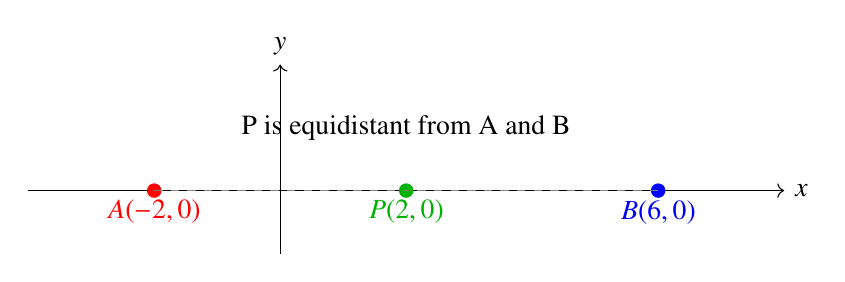
\begin{tikzpicture}[scale=0.8]
    % Draw axes
    \draw[->] (-4,0) -- (8,0) node[right] {$x$};
    \draw[->] (0,-1) -- (0,2) node[above] {$y$};

    % Plot points
    \filldraw[red] (-2,0) circle (3pt) node[below] {$A(-2,0)$};
    \filldraw[blue] (6,0) circle (3pt) node[below] {$B(6,0)$};
    \filldraw[green!70!black] (2,0) circle (3pt) node[below] {$P(2,0)$};

    % Draw dashed lines showing equal distance
    \draw[dashed, gray] (-2,0) -- (2,0);
    \draw[dashed, gray] (6,0) -- (2,0);

    % Add label
    \node at (2,1) {P is equidistant from A and B};
\end{tikzpicture}
\end{center}
\end{frame}

\end{document}